\documentclass[11pt,a4paper]{ltjsarticle}
\usepackage{luatexja}
\usepackage{luatexja-fontspec}
\usepackage{amsmath,amssymb}
\usepackage{graphicx}
\usepackage{longtable,booktabs,array}
\usepackage{float}
\usepackage[margin=25mm]{geometry}
\usepackage{caption}
\usepackage{hyperref}
\hypersetup{colorlinks=true,linkcolor=blue,urlcolor=blue,citecolor=blue}
\setkeys{Gin}{width=0.82\linewidth,keepaspectratio}
\usepackage{amsthm}
\newtheorem{theorem}{定理}
\newtheorem{proposition}{命題}
\newtheorem{lemma}{補題}
\newtheorem{corollary}{系}
\newtheorem{definition}{定義}
\newtheorem{remark}{注意}
\newtheorem{observation}{観察}
\usepackage{calc}
\newcounter{none}
\providecommand{\real}[1]{#1}
\providecommand{\pandocbounded}[1]{#1}
\providecommand{\tightlist}{\setlength{\itemsep}{0pt}\setlength{\parskip}{0pt}}
\title{局在奇数倍音ダブルスリット模型における de Broglie 波長の模擬観測}
\author{木原 範昭 (Noriaki Kihara), WF System Co., Ltd.~--- DOI:
10.5281/zenodo.21109903}
\date{v0.3 --- 2026年7月}
\begin{document}
\maketitle
\emph{------ 高局在構造の干渉生存条件と、観測波長の基本波長不変性}

\section{要旨}\label{ux8981ux65e8}

de Broglie 波長 \(\lambda=h/p\) は、Davisson--Germer の1927年電子回折
{[}2{]}
で確認された。本稿は、この関係を\textbf{単一源ダブルスリットの古典波動模型}の内部で\textbf{模擬観測}する数値実験である（干渉・整列判定は決定論的で、入力の位置・波長揺らぎのみ独立なモンテカルロで与える）。電子は、代表波長
\(\lambda_0=h/p\) を持ち、\(N>1\)
の等振幅奇数倍音和で構成される\textbf{空間局在波}としてモデル化する
{[}1{]}（後述のとおり、これは電子波束そのものではなく、空間局在パルスを作る最小フーリエ構成の古典的アナログである）。物理スケール（\(L=5\,\mathrm{cm}\),
\(W=5\,\mu\mathrm{m}\)）で厳密な二スリット干渉を計算すると、\(N=1\)
は常に干渉し縞間隔から \(\lambda_0\)
を回収する（＝手続きの検算）。\(N>1\)
では、局在形状が保たれるには倍音間の整列条件（幾何共鳴
\(r_{\mathrm{avg}}/\lambda=M/2\)）を要し、これを満たさない波長では局在が崩壊して安定な縞を成さない。中心波長を
\(\lambda_0=h/p\)
とする対称揺らぎのもとで各電子を厳密に計算すると、安定に干渉する有効波長
\(\lambda'\) が最近接共鳴として選ばれる。\textbf{本稿が示す中心的結果は
\(h\) の値ではない。} 共鳴格子間隔は \(\sim10^{-19}\,\mathrm{m}\)
と極めて密で \(\lambda'\approx\lambda_0\)（相対
\(\sim10^{-9}\)）となり、\(p\lambda'\approx h\)
はほぼ同語反復的な自己整合にすぎない。本稿の重心は、\textbf{\(\lambda_0\)
より細かい局在構造（\(N>1\)
奇数倍音）を詰めても、二スリット幾何で鋭い単一ピーク干渉として''生存''でき、観測される中央縞間隔が基本波長
\(\lambda_0\) のまま（\(N\) は局在の鋭さ \(\sim1/(N{+}1)\)
のみ制御）に保たれる}、という\textbf{構造の干渉生存と観測波長の基本波長不変性}にある。この基本波長不変性は、\(\lambda_0\)
をどの物理的由来の基本波長として与えたかには依存しない\textbf{構造的}結果であり、\(h\)
の数値回復とは別の主張である。\textbf{本稿は \(p\lambda=h\)
の第一原理的導出でも、\(\Delta x\,\Delta p\sim h\)
型不確定性の導出でもない。}
誤読対策として、各電子ごとに源位置（\(\cos^2\),
\(\pm\lambda_0/2\)）と初期波長（\(\cos^2\),
\(\pm1\%\)）を独立に乱択し、各 \((y,\lambda_0')\)
で毎回厳密に干渉・整列・除外判定を行った。中心波長を \(\lambda_0=h/p\)
とする対称揺らぎのもとで、\(\langle p\lambda'\rangle\)
は標準誤差の範囲で \(h\) と一致し（標準偏差 \(\sigma\approx0.36\%\) ＝
\(\cos^2\) 分布の理論値、SE
\(\approx\sigma/\sqrt{n_{\mathrm{OK}}}\)）、\(\lambda_0'\)
が共鳴中間点に落ちる数\%の試行が抽出手続き上除外される。

\begin{center}\rule{0.5\linewidth}{0.5pt}\end{center}

\section{1.
導入と本稿の位置づけ}\label{ux5c0eux5165ux3068ux672cux7a3fux306eux4f4dux7f6eux3065ux3051}

de Broglie は1924--1925年、粒子に波長 \(\lambda=h/p\) を対応させた
{[}3{]}。この関係は Davisson--Germer のニッケル電子回折 {[}2{]}
で確認された（Bragg 条件 \(n\lambda=2d\sin\theta\)、既知 \(d\)・実測
\(\theta\) から \(\lambda\) を得て \(h/p\) と照合）。

本稿の位置づけを明確にする。

\begin{itemize}
\tightlist
\item
  \textbf{新しい実験手法の提案でも、実在実験の再測定でもない。}
\item
  \textbf{\(p\lambda=h\) を第一原理から導出するものでもない}（§5.1,
  §5.2）。
\item
  二スリット幾何を借りた\textbf{古典波動の数値実験}であり、「de Broglie
  スケールの代表波長を持つ\textbf{高局在}古典波（\(N>1\)
  奇数倍音）が、二スリット幾何のもとでどのような整列条件を要求し、鋭い干渉として安定に生存できるか、そして観測される波長スケールがどう保たれるか」を調べる。
\end{itemize}

Davisson--Germer
が結晶「格子」を用いたのに対し、本模型はダブルスリットを用いる。ただし実実験では回折角という\textbf{外部測定データ}が
\(\lambda\) を独立に与えるのに対し、本模型は \(\lambda_0=h/p\)
から縞を生成して読み戻すため独立な測定経路を持たない点で同型ではない（§5.3）。本稿の新規性は、{[}1{]}
の局在奇数倍音・整列条件を\textbf{ダブルスリット幾何へ適用}し、\textbf{位置と波長の独立モンテカルロ}のもとで\textbf{各電子ごとの厳密な整列・除外判定}を行い、観測波長の\textbf{基本波長不変性}を統計的に検証した点にある。

\begin{center}\rule{0.5\linewidth}{0.5pt}\end{center}

\section{2.
モデル定義と計算方法}\label{ux30e2ux30c7ux30ebux5b9aux7fa9ux3068ux8a08ux7b97ux65b9ux6cd5}

\subsection{2.1 幾何}\label{ux5e7eux4f55}

源--スリット距離 \(L=5\,\mathrm{cm}\)、スリット間隔
\(W=5\,\mu\mathrm{m}\)、スリットは \(y_{\mathrm{slit}}=\pm W/2\)。源位置
\(y\)（後述で揺らぐ）に対する二経路の距離は
\[r_1(y)=\sqrt{L^2+(y-W/2)^2},\quad r_2(y)=\sqrt{L^2+(y+W/2)^2},\quad r_{\mathrm{avg}}=\tfrac{r_1+r_2}{2}.\]
物理スケールでは特徴長が桁違い（\(W/\lambda_0\sim5\times10^4\),
\(L/W\sim10^4\),
\(L/\lambda_0\sim5\times10^8\)）で共通縮尺の作図は不可能、半角は
\(\theta=\arctan[(W/2)/L]\approx2.9\times10^{-3}{}^\circ\)
と極端に近軸である。

\pandocbounded{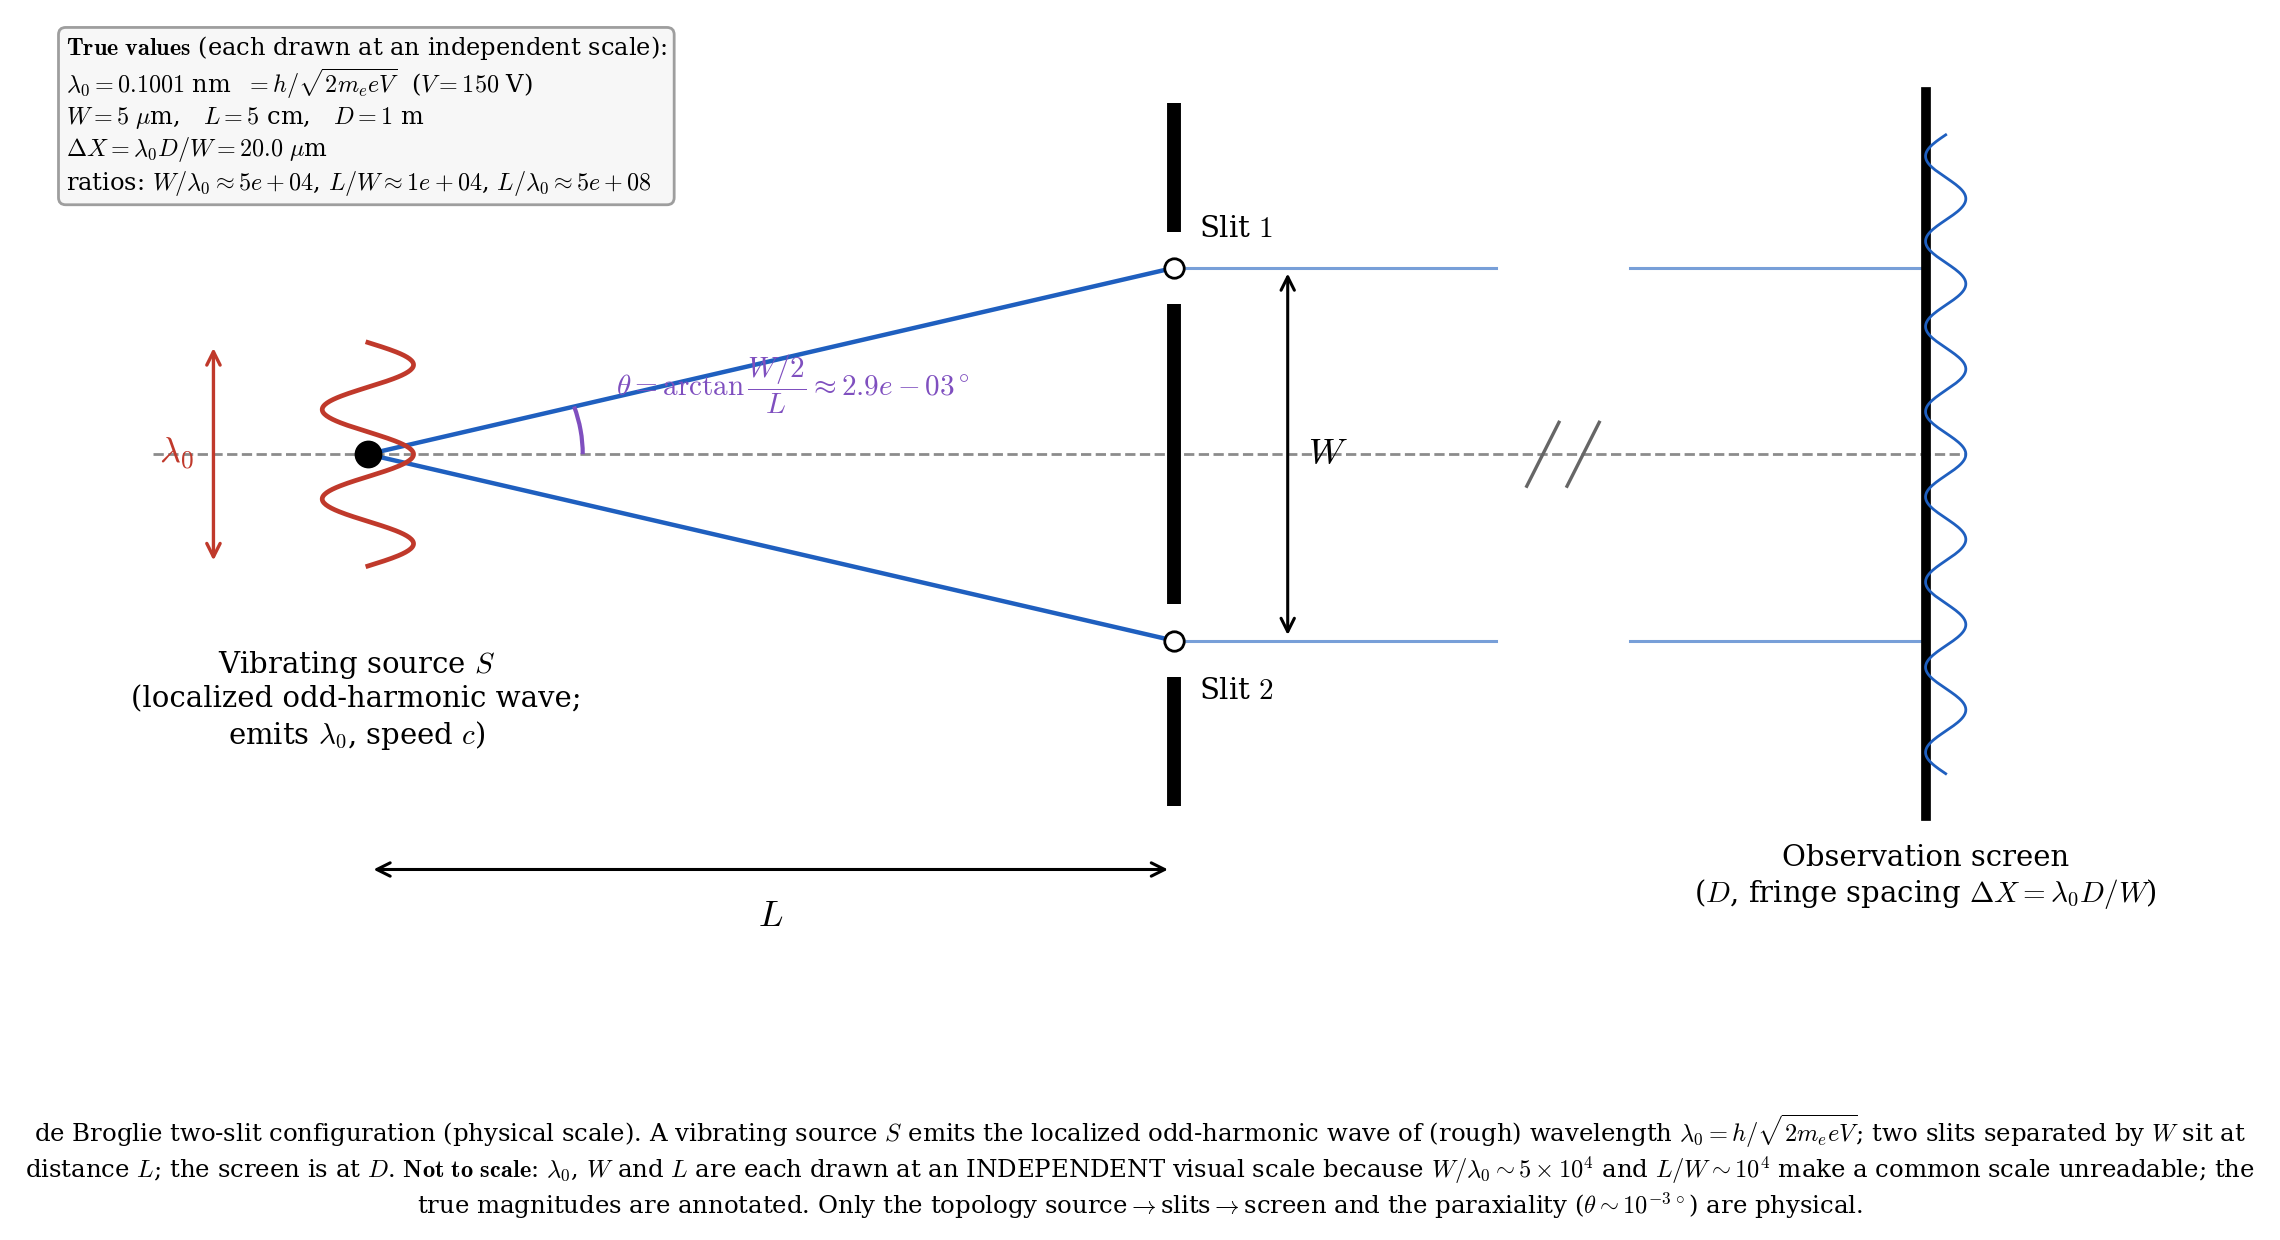
\includegraphics[keepaspectratio,alt={図1}]{fig_setup_debroglie_V150.png}}
\textbf{図1}: 実験系の模式図（\(V=150\,\mathrm{V}\)）。\(\lambda_0,W,L\)
は各々独立の縮尺で描く（左上ボックスに実比
\(W/\lambda_0\approx5\times10^4\) 等）。物理的に正しいのは topology
と近軸性 \(\theta\sim10^{-3\,\circ}\)
のみで、寸法比は誇張されている（本文 §2.1 参照）。

\subsection{2.2
局在奇数倍音波と厳密強度}\label{ux5c40ux5728ux5947ux6570ux500dux97f3ux6ce2ux3068ux53b3ux5bc6ux5f37ux5ea6}

\textbf{物理的動機}：以下では便宜上「電子」と呼ぶが、本稿で計算するのは電子の完全な量子状態ではなく、de
Broglie
スケールを代表波長とする古典局在波の試行である。本模型は、その局在波を、空間的な拡がりを持たない点でなく\textbf{空間局在パルス波}として扱う。等振幅の奇数倍音和は、中央
\(s=0\) に対称な局在ピークを与える最小のフーリエ構成であり
{[}1{]}、偶数成分を除くことで対称性が保たれる。\textbf{注意}：この奇数倍音成分は、標準量子力学における自由電子の異なる運動量固有状態（波数
\(n\) 倍は運動量 \(np\)・エネルギー
\(n^2E\)）をそのまま意味するものではなく、\textbf{局在波形を構成するための古典波動模型上のフーリエ成分}である。また本稿は時間発展を含む量子波束模型ではなく、\textbf{スクリーン上の空間位相構造を検査する定常古典波動模型}であり、倍音間のエネルギー分散や時間的デコヒーレンスは対象外とする。

波数成分 \(n=1,3,\dots,N\)（\(\lambda_n=\lambda/n\)、\(K=(N{+}1)/2\)
本）。二スリットを経たスクリーン上の厳密強度は
\[I(s;y)=\Big|\sum_{n=1,3,\dots,N}\big(e^{i\Phi_1^{(n)}}+e^{i\Phi_2^{(n)}}\big)\Big|^2,\qquad
\Phi_k^{(n)}=\frac{2\pi n}{\lambda}\big(r_k-y_{\mathrm{slit},k}\,s\big),\]
ここで \(s\) はスクリーン方向の近軸変数（遠方座標 \(X\) に対し
\(s\simeq X/D\)）。数値的には代数的に等価な因子化形
\[e^{i\Phi_1^{(n)}}+e^{i\Phi_2^{(n)}}=e^{i\,2\pi n\,r_{\mathrm{avg}}/\lambda}\cdot2\cos\!\Big(\pi n\frac{(r_1-r_2)-Ws}{\lambda}\Big),\quad r_1-r_2=\frac{-2Wy}{r_1+r_2}\]
を用いる（物理は不変、絶対位相 \(\sim10^9\,\mathrm{rad}\)
での桁落ちを回避）。\textbf{この形では、\(e^{i2\pi n r_{\mathrm{avg}}/\lambda}\)
が倍音間の絶対整列を担い、\(\cos(\pi n[(r_1-r_2)-Ws]/\lambda)\)
が二経路干渉の相対位相を担う。}
すなわち、通常の二重スリットで観測される主因は経路差（相対位相）だが、本模型では局在奇数倍音波形を中央で保つために\textbf{追加で絶対平均距離
\(r_{\mathrm{avg}}\) に対する倍音整列}が要る。

\subsection{\texorpdfstring{2.3 中央整列度
\(A(\lambda)\)（絶対指標）}{2.3 中央整列度 A(\textbackslash lambda)（絶対指標）}}\label{ux4e2dux592eux6574ux5217ux5ea6-alambdaux7d76ux5bfeux6307ux6a19}

スクリーン中央 \(s=0\) の強度は
\(I(0)=\big|2\sum_n e^{i2\pi n r_{\mathrm{avg}}/\lambda}\big|^2=4K^2A(\lambda)\)、
\[A(\lambda)=\frac{1}{K^2}\Big|\sum_{n=1,3,\dots,N}e^{i2\pi n\,r_{\mathrm{avg}}/\lambda}\Big|^2.\]
\(A\)
は\textbf{完全整列の割合}である：\(A=1\)（\(I(0)=4K^2\)）は全奇数倍音位相が揃った真の共鳴（\(r_{\mathrm{avg}}/\lambda=M/2\)）のときのみで、それ以外は
\(A<1\)。前節のとおり \(A\)
は上式（絶対整列）の指標であり、\textbf{局在波形の保存条件}を測る。\(A\)
は幾何と \(N\) で決まる絶対最大 \(4K^2\)
を基準とするため、部分整列した劣化パターンは \(A\ll1\)
として正しく棄却される（自己正規化 \(I(0)/I_{\max}\)
ではこの識別ができない）。

\subsection{2.4
各電子ごとの独立な揺らぎと忠実計算}\label{ux5404ux96fbux5b50ux3054ux3068ux306eux72ecux7acbux306aux63faux3089ux304eux3068ux5fe0ux5b9fux8a08ux7b97}

実在装置の揺らぎを模し、\textbf{各電子（各試行）ごとに2つの独立なモンテカルロ乱択}を与える：

\begin{enumerate}
\def\labelenumi{\arabic{enumi}.}
\tightlist
\item
  \textbf{源位置} \(y\sim\cos^2(\pi y/\Delta)\)、範囲
  \(\pm\Delta/2\)（\(\Delta=\lambda_0\)、中央 \(0\) がピーク）。
\item
  \textbf{初期波長}
  \(\lambda_0'=\lambda_0+\eta\)、\(\eta\sim\cos^2(\pi\eta/2\delta)\)、\(\delta=0.01\,\lambda_0\)（\(\pm1\%\)、上とは別の乱数）。
\end{enumerate}

2つは別々に乱択するので無相関（位置と波長に誤った相関が入らない）。各電子について、その
\((y,\lambda_0')\) の幾何 \(r_{\mathrm{avg}}(y)\)
を用いて\textbf{毎回厳密に}干渉・整列・除外判定を行う（\(y=0\)
固定・\(\lambda_0\) 固定の近似はしない；\(N=9\)・電圧1点あたり約
\(4\times10^4\) 回の \(A\) 評価）。\(\cos^2\) 分布の理論標準偏差は
\(\sigma=\delta\sqrt{1/3-2/\pi^2}\approx0.362\,\delta\)、すなわち
\(\pm1\%\) 入力に対し \textbf{\(\sigma\approx0.362\%\)}。

\subsection{\texorpdfstring{2.5 有効波長 \(\lambda'\)
の探索と除外判定}{2.5 有効波長 \textbackslash lambda\textquotesingle{} の探索と除外判定}}\label{ux6709ux52b9ux6ce2ux9577-lambda-ux306eux63a2ux7d22ux3068ux9664ux5916ux5224ux5b9a}

各電子について、\(\lambda_0'\) 近傍の\textbf{幾何窓}
\([\lambda_0'-\lambda_0'^2/(4r_{\mathrm{avg}}),\ \lambda_0'+\lambda_0'^2/(4r_{\mathrm{avg}})]\)（＝半共鳴間隔）内で
\(A(\lambda)\) を掃引し、\(A\ge0.98\)
の連結帯（共鳴帯）を数える。帯がちょうど1つなら黄金分割でそのピークを精密化して有効波長
\(\lambda'=2r_{\mathrm{avg}}/M\) を得る（\(A(\lambda')=1\),
\(I(0)=4K^2\) を機械精度で満たす）。帯が0本または2本以上（\(\lambda_0'\)
が共鳴中間点近傍で最近接共鳴が一意でない）なら、その試行を除外する。窓幅・整列条件は幾何のみで決まり、\(h\)
は \(\lambda_0'\) の中心 \(\lambda_0=h/p\)
を通してしか入らない。観測次数
\(M=\mathrm{round}(2r_{\mathrm{avg}}/\lambda')\)
は事後出力である（次数の記号 \(M\) は電子質量 \(m_e\) と区別する）。

\textbf{「整列（スナップ）」の物理的解釈（重要）}：本模型の整列は、源が放射後に波長を物理的に変える機構（例：スリットからの後方散乱による引き込み＝injection
locking）を主張するものではない。それは、\textbf{「整列する波長のみが安定な単一ピーク縞を形成し、それ以外は縞を成さない」という生存バイアス（フィルタリング）を数学的に代行する操作}である。除外（前段落の
``帯 ≠ 1''
の試行）はこのフィルタの一部（最近接共鳴を一意に選べない試行の除去）であり、\textbf{閾値
0.98
と窓幅に依存する手続き的判定}であって、物理的に電子が消失することを意味しない（率は自然でなく閾値が決める）。本稿でいう「生存」とは、安定した単一ピーク縞として抽出可能であることを指し、物理的な電子の生死を意味しない。なお、主ピーク間隔は整列共鳴
\(\lambda'=2r_{\mathrm{avg}}/M\) で決まるため、閾値 \(A\ge0.98\)
を変えても原理的には除外率が主に変わるだけで、align
後の主ピーク間隔の不変性（§4）は保たれると考えられる（閾値変化の系統的検証は今後の課題）。

\subsection{\texorpdfstring{2.6 \(\lambda_0\) の役割と \(N=1\)／\(N>1\)
の位置づけ}{2.6 \textbackslash lambda\_0 の役割と N=1／N\textgreater1 の位置づけ}}\label{lambda_0-ux306eux5f79ux5272ux3068-n1n1-ux306eux4f4dux7f6eux3065ux3051}

\(\lambda_0=h/p\) は干渉計算の初期条件であり、\(\lambda_0\) なしには位相
\(2\pi r/\lambda\) が定義できない。\(\lambda_0\) 自体が \(h\)
を用いて与えられる以上、\(p\lambda'\) の回復は \(h\)
の独立導出ではなく自己整合的検証である。

\begin{itemize}
\tightlist
\item
  \textbf{\(N=1\)（単一倍音）}
  は整列条件を要さず常に干渉し、縞間隔から同じ \(\lambda_0\)
  が回収される。したがって \(N=1\)
  は物理的発見でなく、\textbf{計算と波長読み取り手続きの検算}である。
\item
  \textbf{\(N>1\)（局在奇数倍音波）} が主眼である。この波形は
  \(\lambda_0\) より細かい局在構造を持ち、安定に干渉できるのは離散共鳴
  \(r_{\mathrm{avg}}/\lambda=M/2\) 上に限られる（§2.2
  の絶対整列条件）。電子の \(\lambda_0\)
  は一般にこの格子に乗らないため、そのままでは崩壊し、\(A\) 最大の
  \(\lambda'\)（最近接共鳴）が生存フィルタにより選ばれる。
\end{itemize}

物理スケールでは共鳴格子間隔
\(\lambda_0^2/(2r_{\mathrm{avg}})\sim10^{-19}\,\mathrm{m}\)
が極めて密で、\(\lambda'\) は \(\lambda_0\) に相対 \(\sim10^{-9}\)
で一致する。したがって「\(\lambda'\)
が微調整される」こと自体は同語反復であり、そこに新しい物理はない。\textbf{\(N>1\)
が示す固有の内容は、値の回復ではなく、次の2点である}：(i) \(\lambda_0\)
より細かい局在構造を持つ古典波が二スリット幾何で\textbf{鋭い単一ピーク干渉として安定に生存できる}こと、(ii)
生存した縞の\textbf{中央間隔が基本波長 \(\lambda_0\) のままで倍音数
\(N\) によらない}（\(N\) は局在の鋭さ \(\sim1/(N{+}1)\)
のみ制御する）こと。これらは、\(\lambda_0\)
をどの物理的由来の基本波長として与えたかには依存しない構造的結果であり、\(h\)
の数値回復とは別の主張である。

\begin{center}\rule{0.5\linewidth}{0.5pt}\end{center}

\section{\texorpdfstring{3.
\(N=1\)：ベースライン（手続きの検算）}{3. N=1：ベースライン（手続きの検算）}}\label{n1ux30d9ux30fcux30b9ux30e9ux30a4ux30f3ux624bux7d9aux304dux306eux691cux7b97}

\(N=1\) は無条件に干渉する。各電圧
\(V=50\text{–}500\,\mathrm{V}\)（\(\lambda_0=0.055\text{–}0.173\,\mathrm{nm}\)）で、\(\pm\lambda_0/2\)
の位置揺らぎと \(\pm1\%\)
の波長揺らぎを与えた電子群の厳密二スリット縞を積算し（図2）、縞間隔から波長を回収する。\(\langle p\lambda\rangle\)
の傾きは \(h\) に対し \(\mathrm{slope}/h=0.99977\)（\(\pm1\%\) 入力を
\(M=200\) 平均した統計残差 \(\sim2\times10^{-4}\)）で一致する。

\pandocbounded{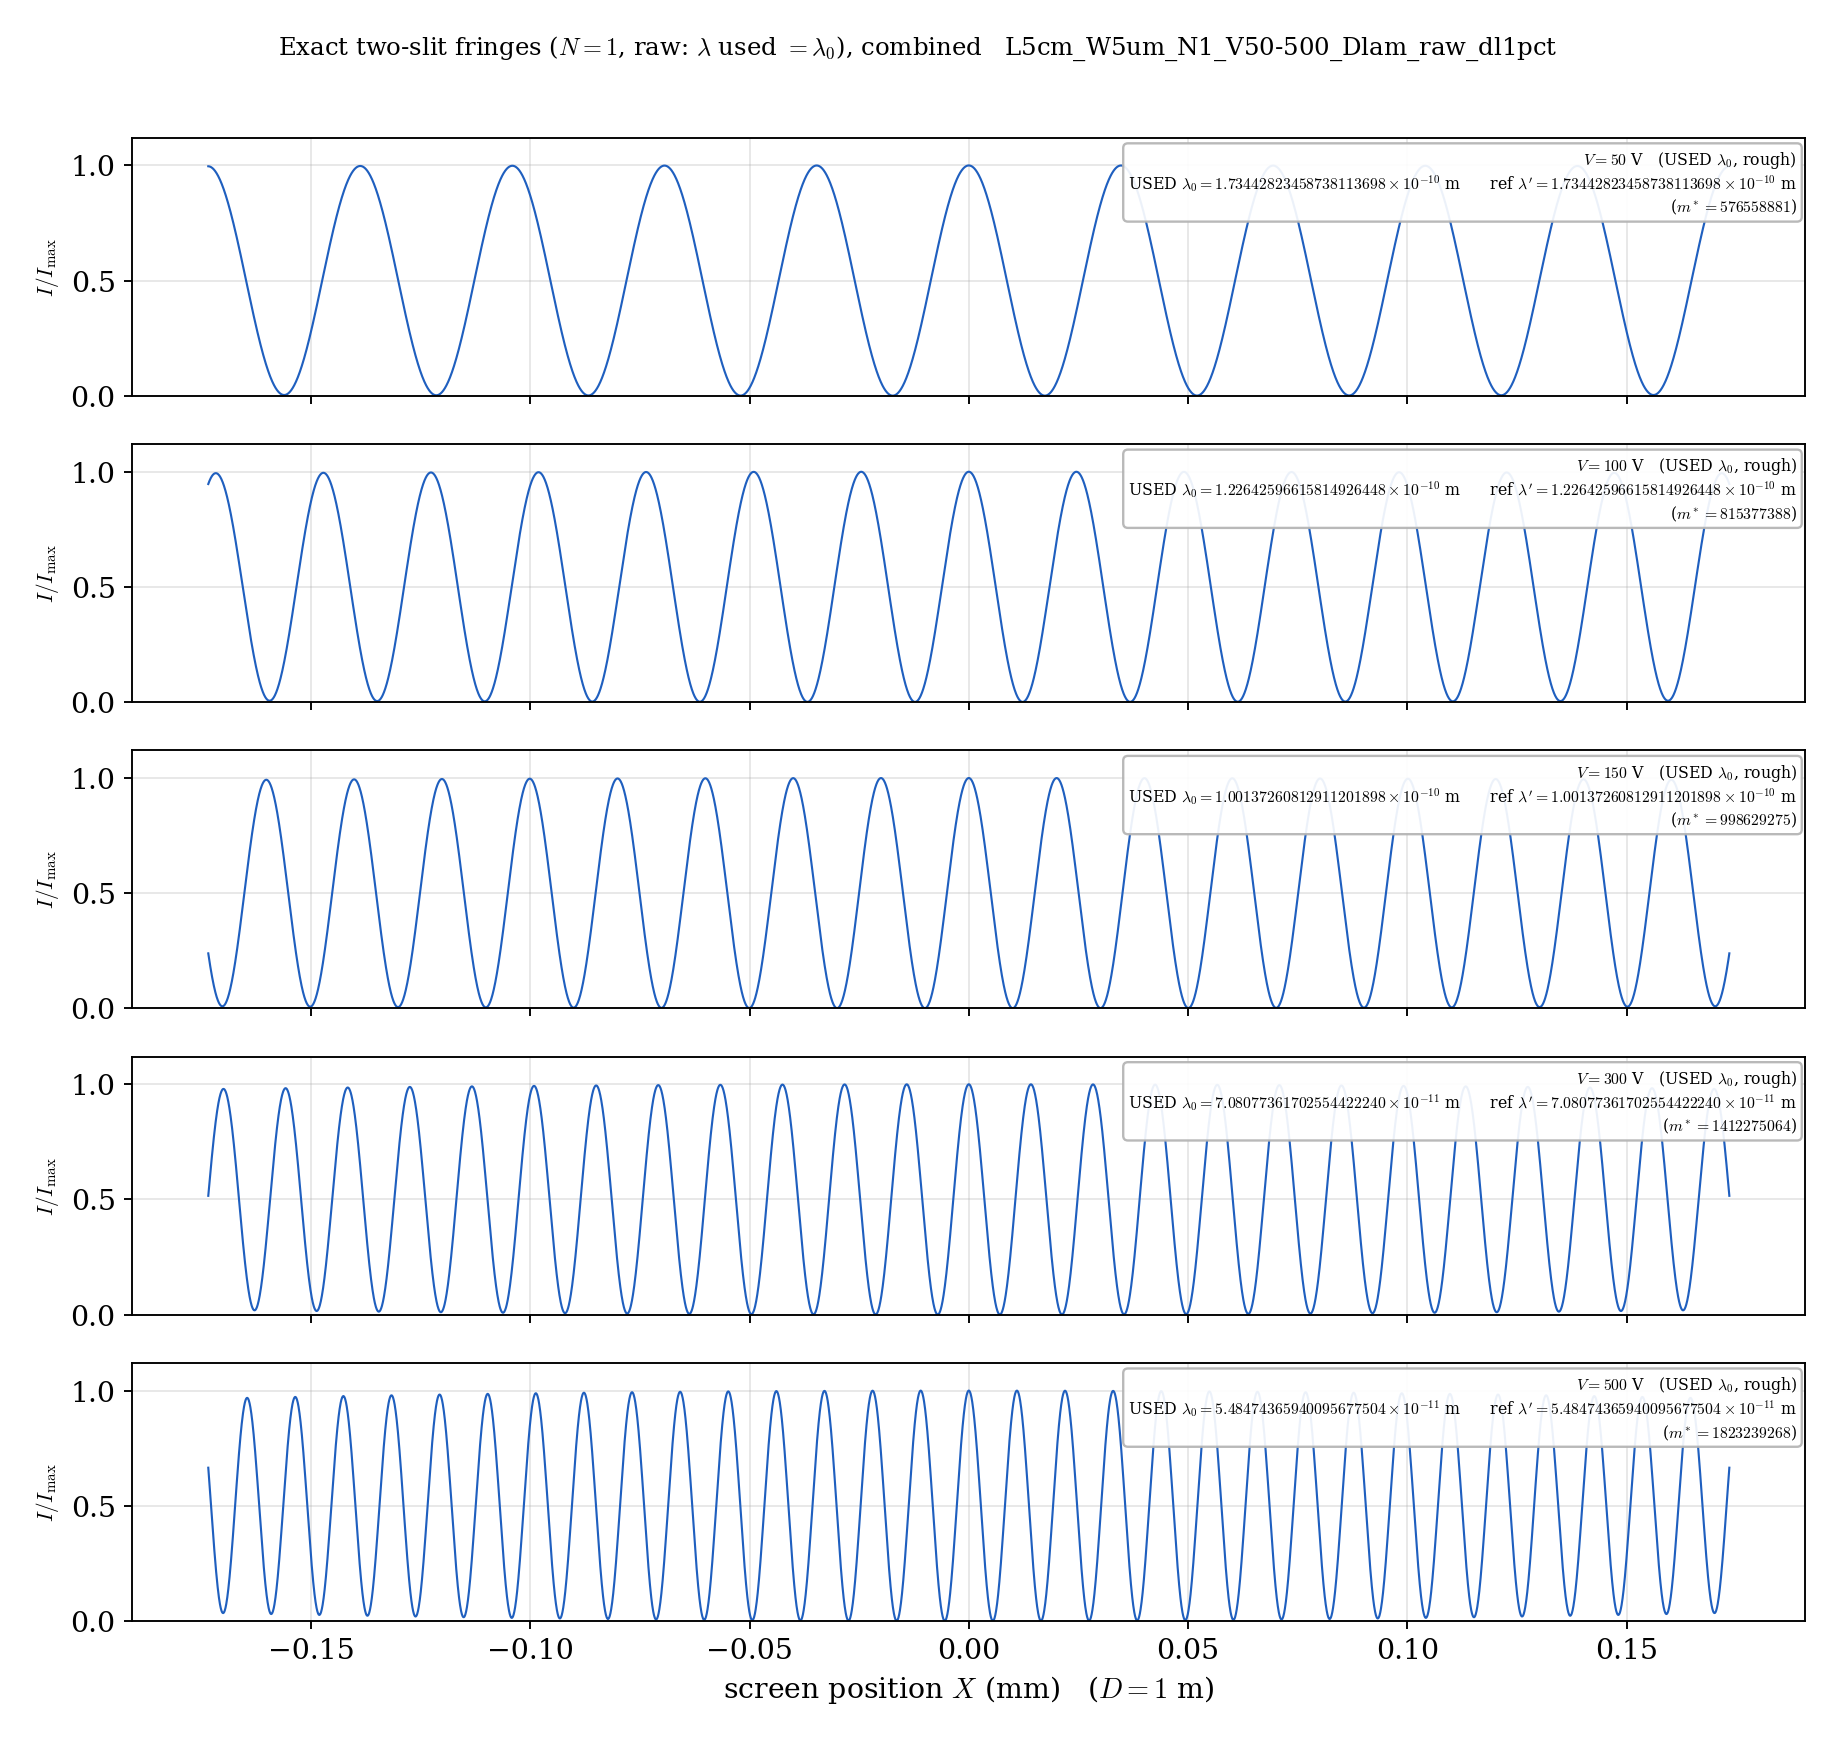
\includegraphics[keepaspectratio,alt={図2}]{debroglie_fringes_combined_L5cm_W5um_N1_V50-500_Dlam_raw_dl1pct.png}}
\textbf{図2}: \(N=1\)
の積算縞（\(V=50,100,150,300,500\,\mathrm{V}\)、\(D=1\,\mathrm{m}\)、共通窓）。各段は、\(\pm\lambda_0/2\)
で揺らぐ源位置と \(\pm1\%\) で揺らぐ波長を持つ 200
電子を厳密に再計算して積算したもの。高電圧ほど縞が詰まり（\(\Delta X=0.035\to0.011\,\mathrm{mm}\)）、\(\pm1\%\)
の波長差により窓の端へ向かうほど僅かに可視度が低下する（本文 §3）。

\begin{center}\rule{0.5\linewidth}{0.5pt}\end{center}

\section{\texorpdfstring{4.
\(N>1\)：干渉の生存と、観測波長の基本波長不変性}{4. N\textgreater1：干渉の生存と、観測波長の基本波長不変性}}\label{n1ux5e72ux6e09ux306eux751fux5b58ux3068ux89b3ux6e2cux6ce2ux9577ux306eux57faux672cux6ce2ux9577ux4e0dux5909ux6027}

多重倍音 \(N=9,17\) を計算する（表1）。

\textbf{未補正（raw, \(\lambda_0'\)
をそのまま使用）}：倍音間の絶対整列位相（\(r_{\mathrm{avg}}/\lambda\sim5\times10^8\)）は一般に揃わず、局在は崩れて多重分裂する。多重ピークのため\textbf{一意な周期が定まらず、縞間隔から波長を読み取れない}。同じ読み取り手続きを形式的に適用した
\(\mathrm{slope}/h\) は \(N=9\): \(0.139\)、\(N=17\): \(0.081\)
だが、\textbf{これは安定縞が存在しない崩壊パターンに対する診断量であり、有効な波長測定値を意味しない}。

\pandocbounded{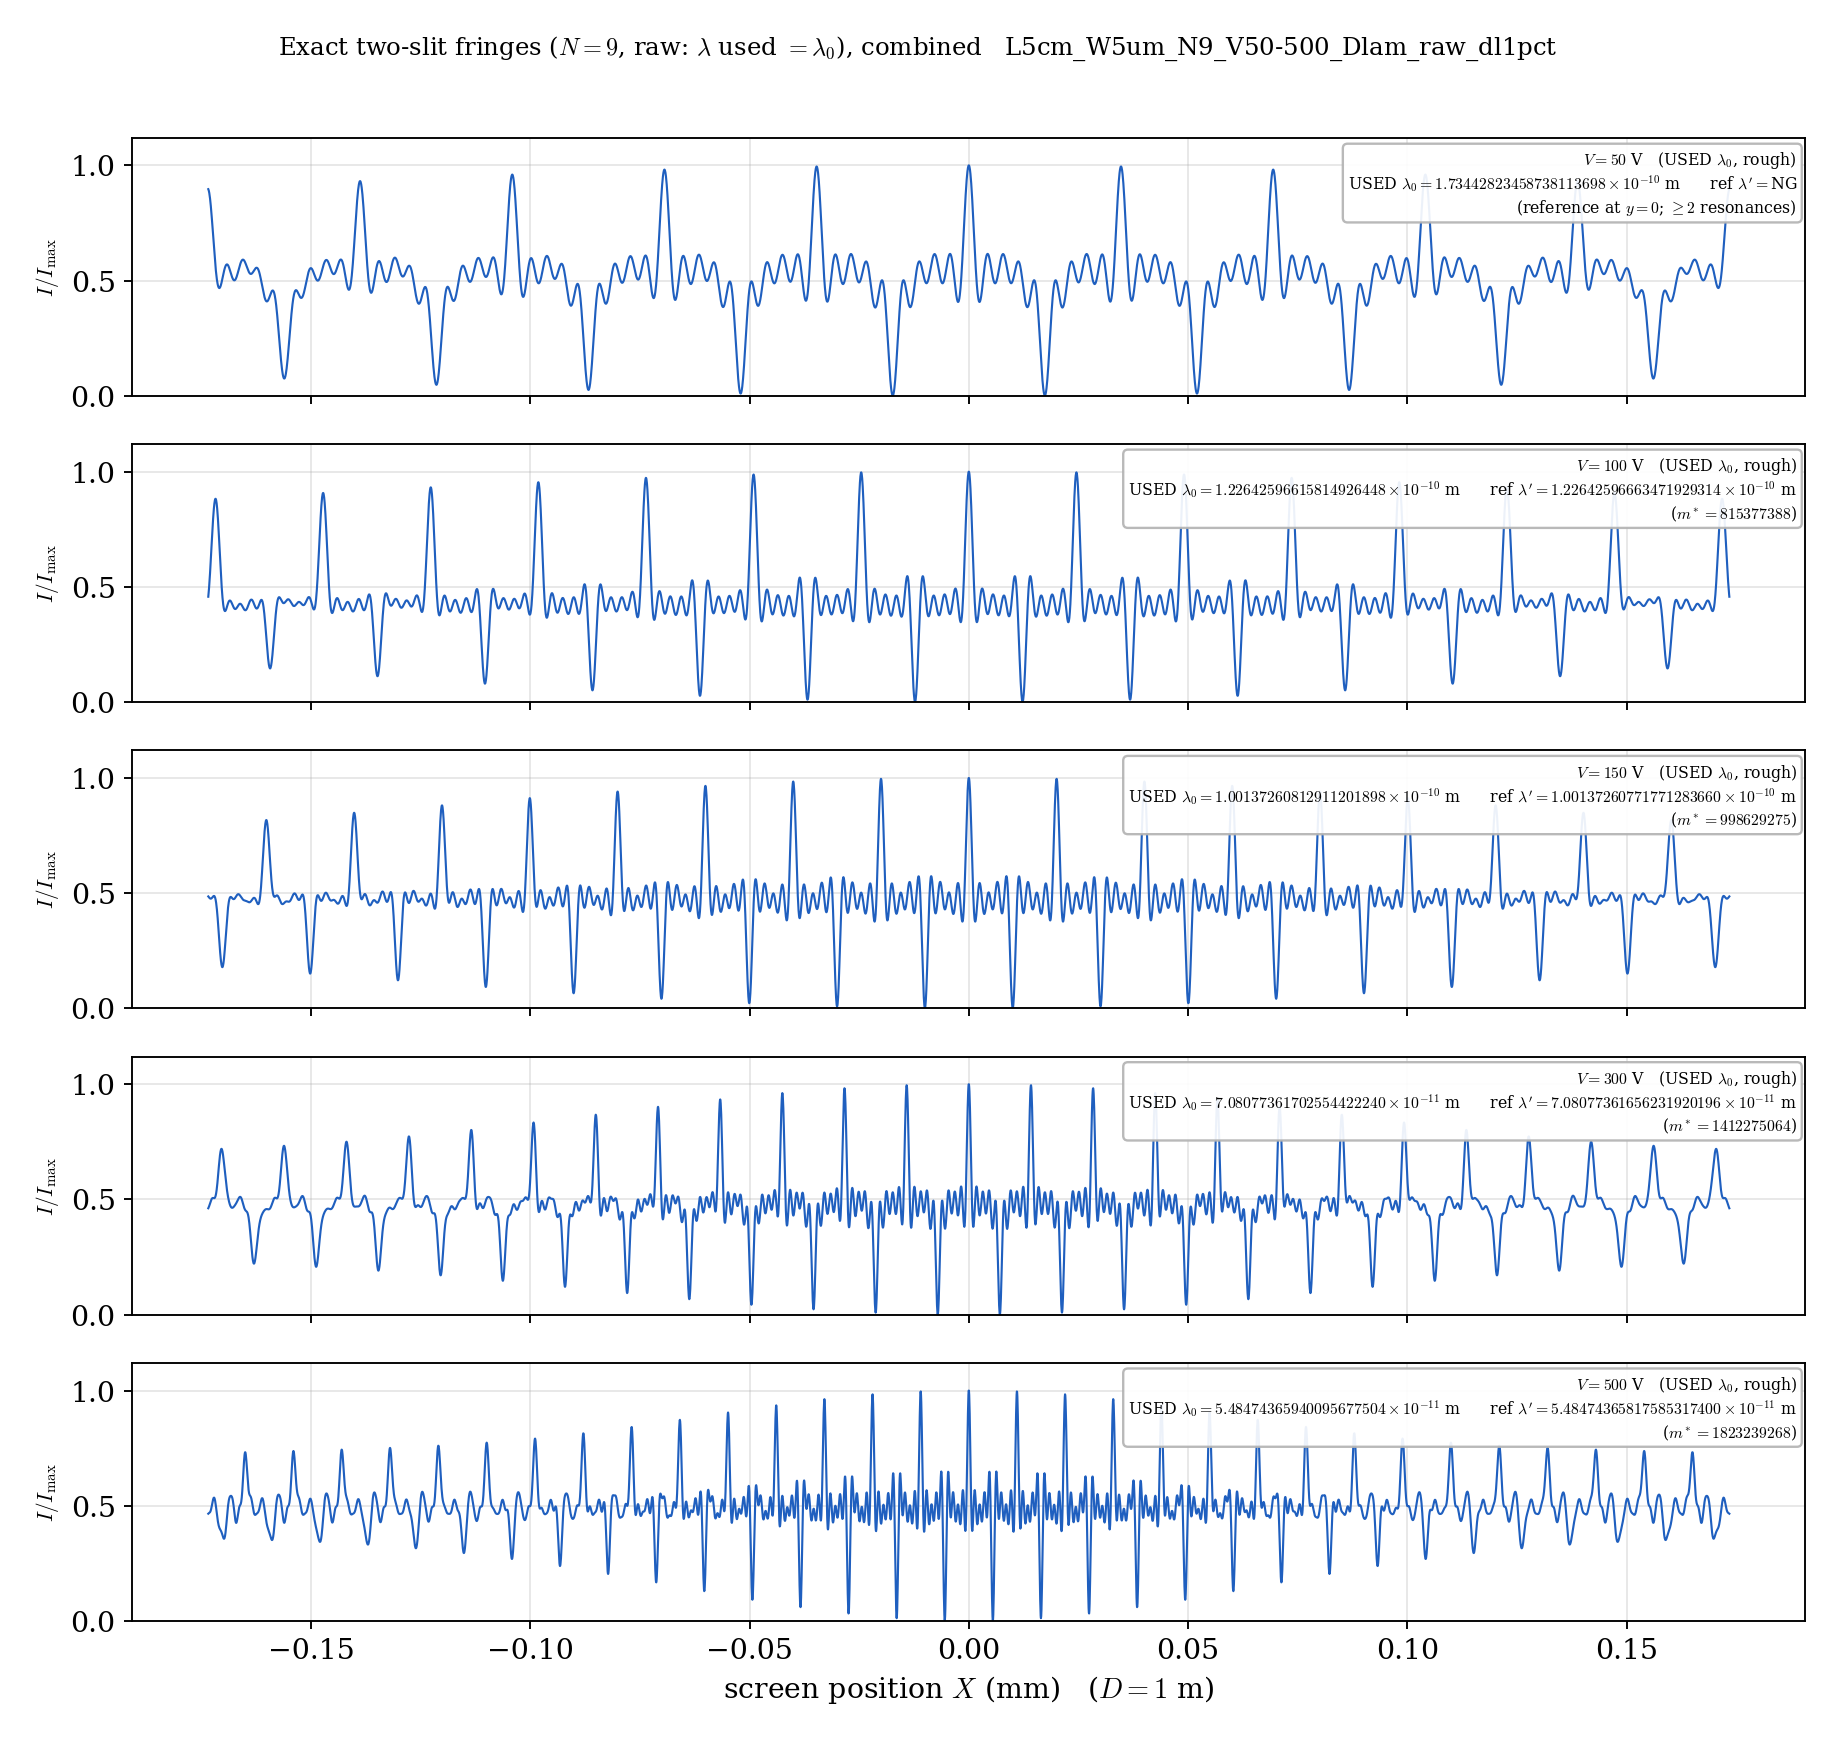
\includegraphics[keepaspectratio,alt={図3}]{debroglie_fringes_combined_L5cm_W5um_N9_V50-500_Dlam_raw_dl1pct.png}}
\textbf{図3}:
\(N=9\)・\textbf{未補正}（raw）の積算縞。各周期が単一ピークにならず\textbf{分裂した多重ピーク（櫛状）}になり、中央
\(s=0\)
が主ピークにならない＝安定干渉が成立していない。この状態では一意な周期が読めない。

\textbf{補正（align, \(\lambda'\) を使用）}：各電子の \(\lambda_0'\)
を、その幾何 \(r_{\mathrm{avg}}(y)\) の最近接共鳴
\(\lambda'=2r_{\mathrm{avg}}/M\)
に整列（＝生存フィルタ、§2.5）。全倍音位相が揃い、鋭い単一局在ピーク列が復活する（図4）。この鋭い列の\textbf{主ピーク間隔
\(\Delta X\) から \(\lambda=\Delta X\cdot W/D\)
として波長を幾何的に読み取ると、\(A\) 経由の \(\lambda'\)
と一致する}（raw では読めなかった波長が align
で回収できる）。\(\langle p\lambda'\rangle\) の傾きは \(N=9\):
\(0.99973\)、\(N=17\): \(0.99972\)。

\pandocbounded{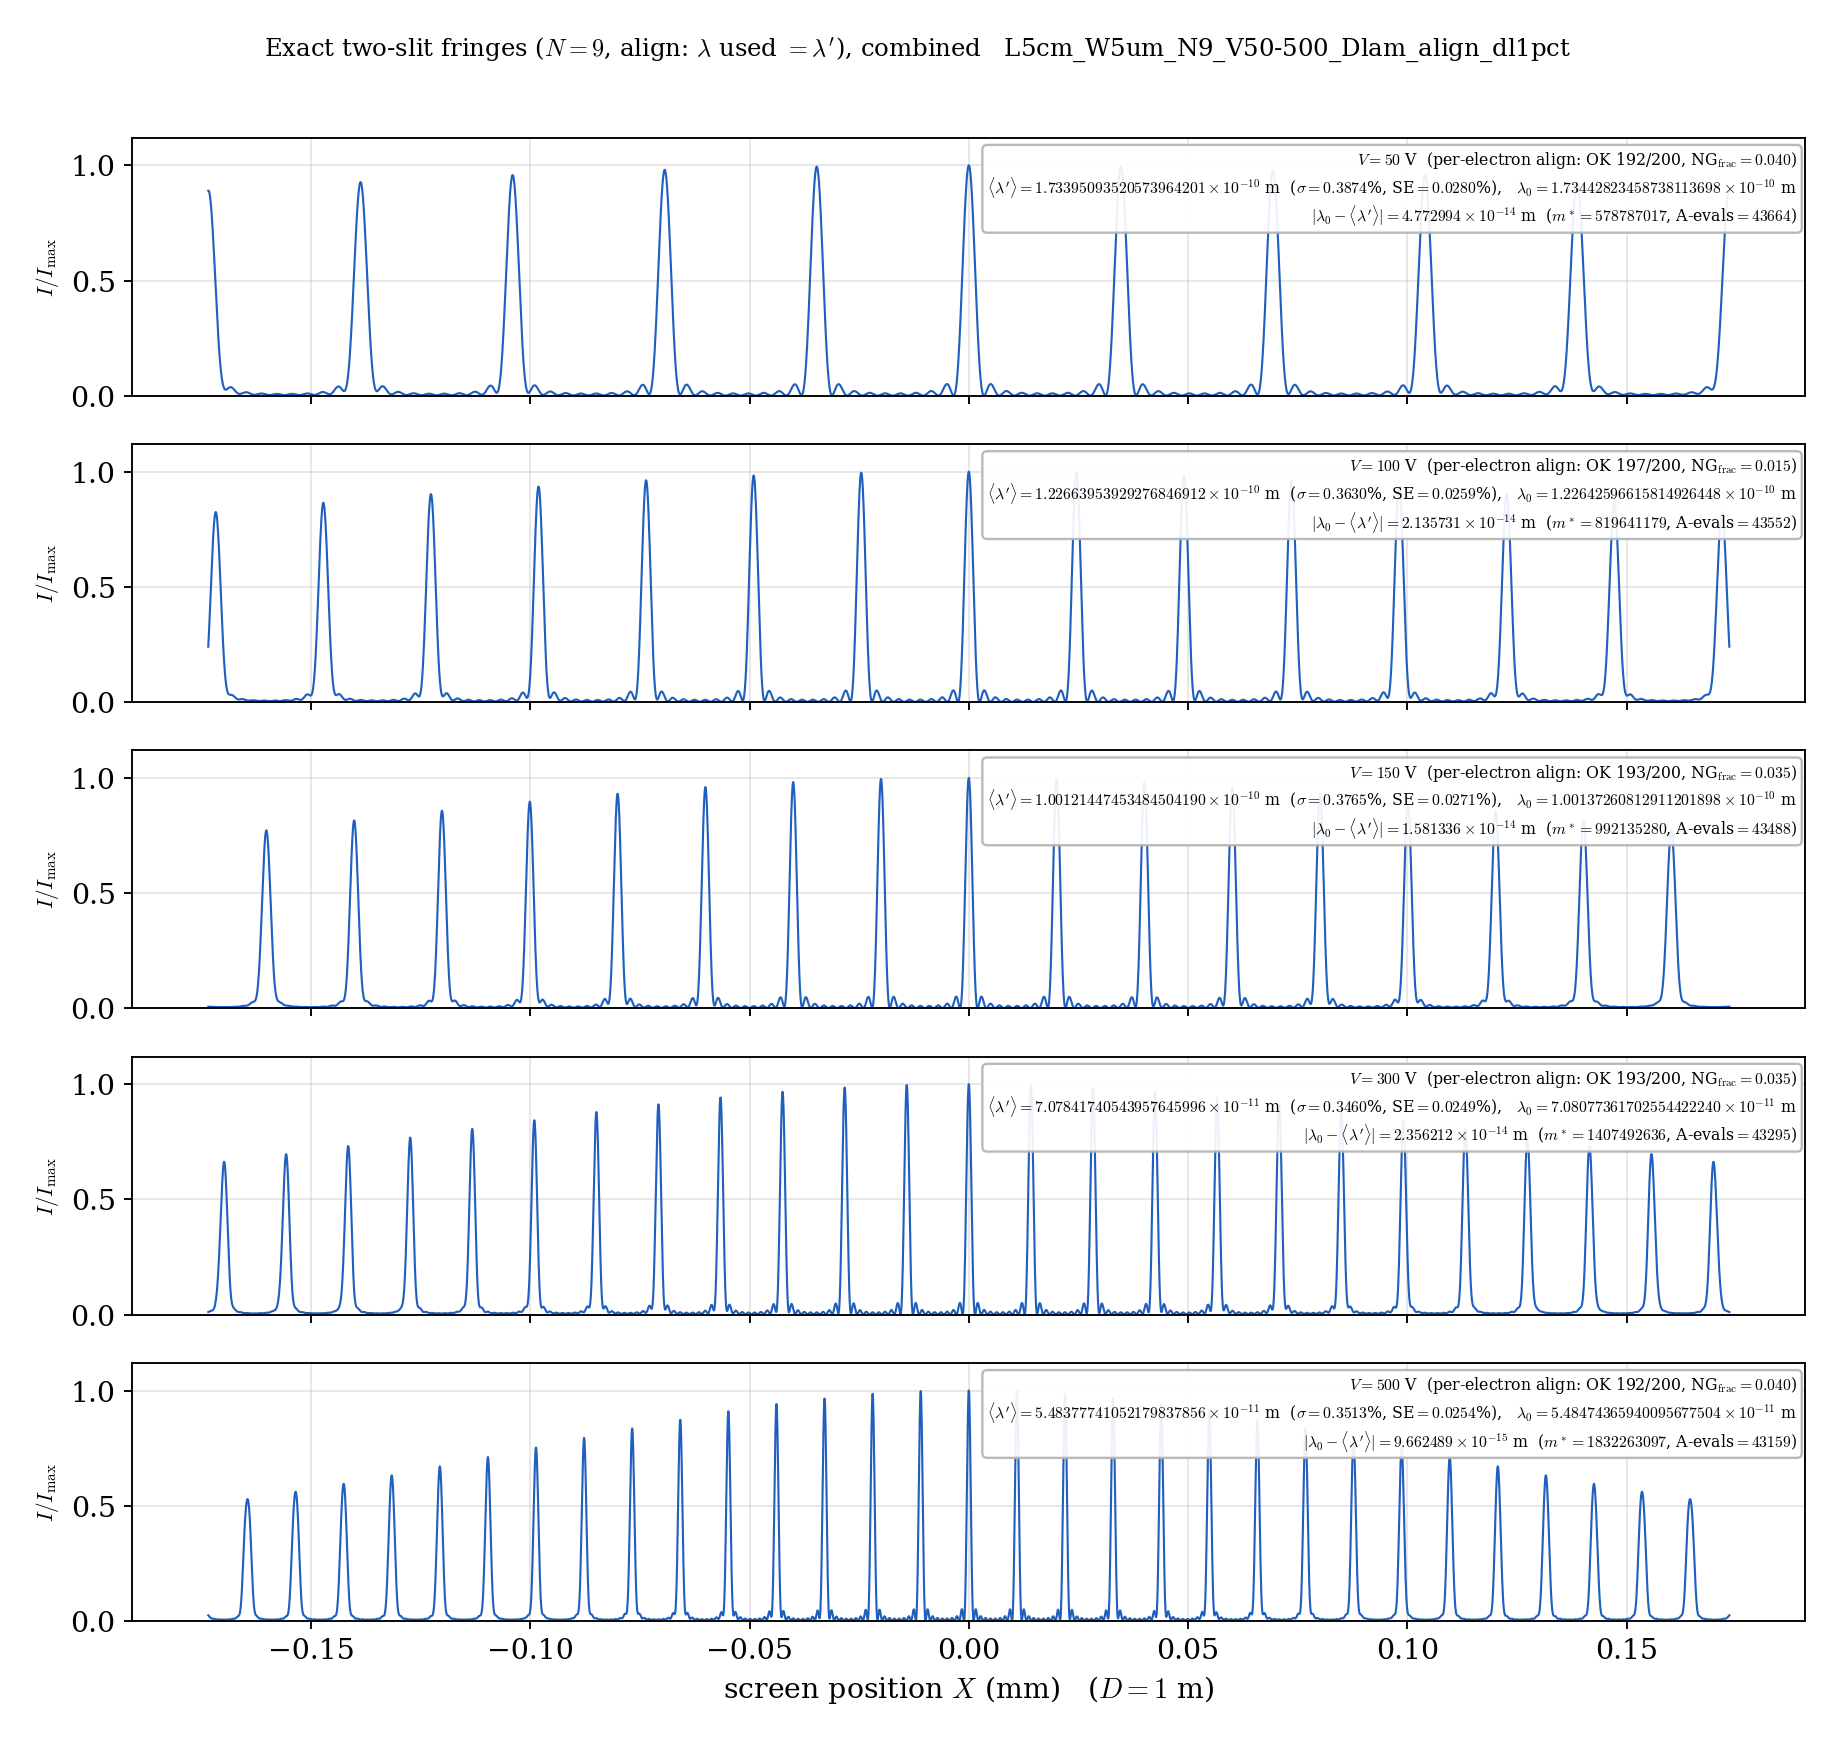
\includegraphics[keepaspectratio,alt={図4}]{debroglie_fringes_combined_L5cm_W5um_N9_V50-500_Dlam_align_dl1pct.png}}
\textbf{図4}:
\(N=9\)・\textbf{整列}（align）の積算縞。図3の櫛状分裂が、生存フィルタにより
\textbf{鋭い単一局在ピーク（\(S_N\) のサイドローブ付き）}
に変わる。各パネル注記に
\(n_{\mathrm{OK}}/200\)、除外率、\(\langle\lambda'\rangle\)（20桁）、\(\sigma\%\)、SE\(\%\)。\(\lambda'\)
は \(\lambda_0\) に相対 \(\sim10^{-9}\)
で一致し、整列は幾何共鳴への微小スナップである。

\pandocbounded{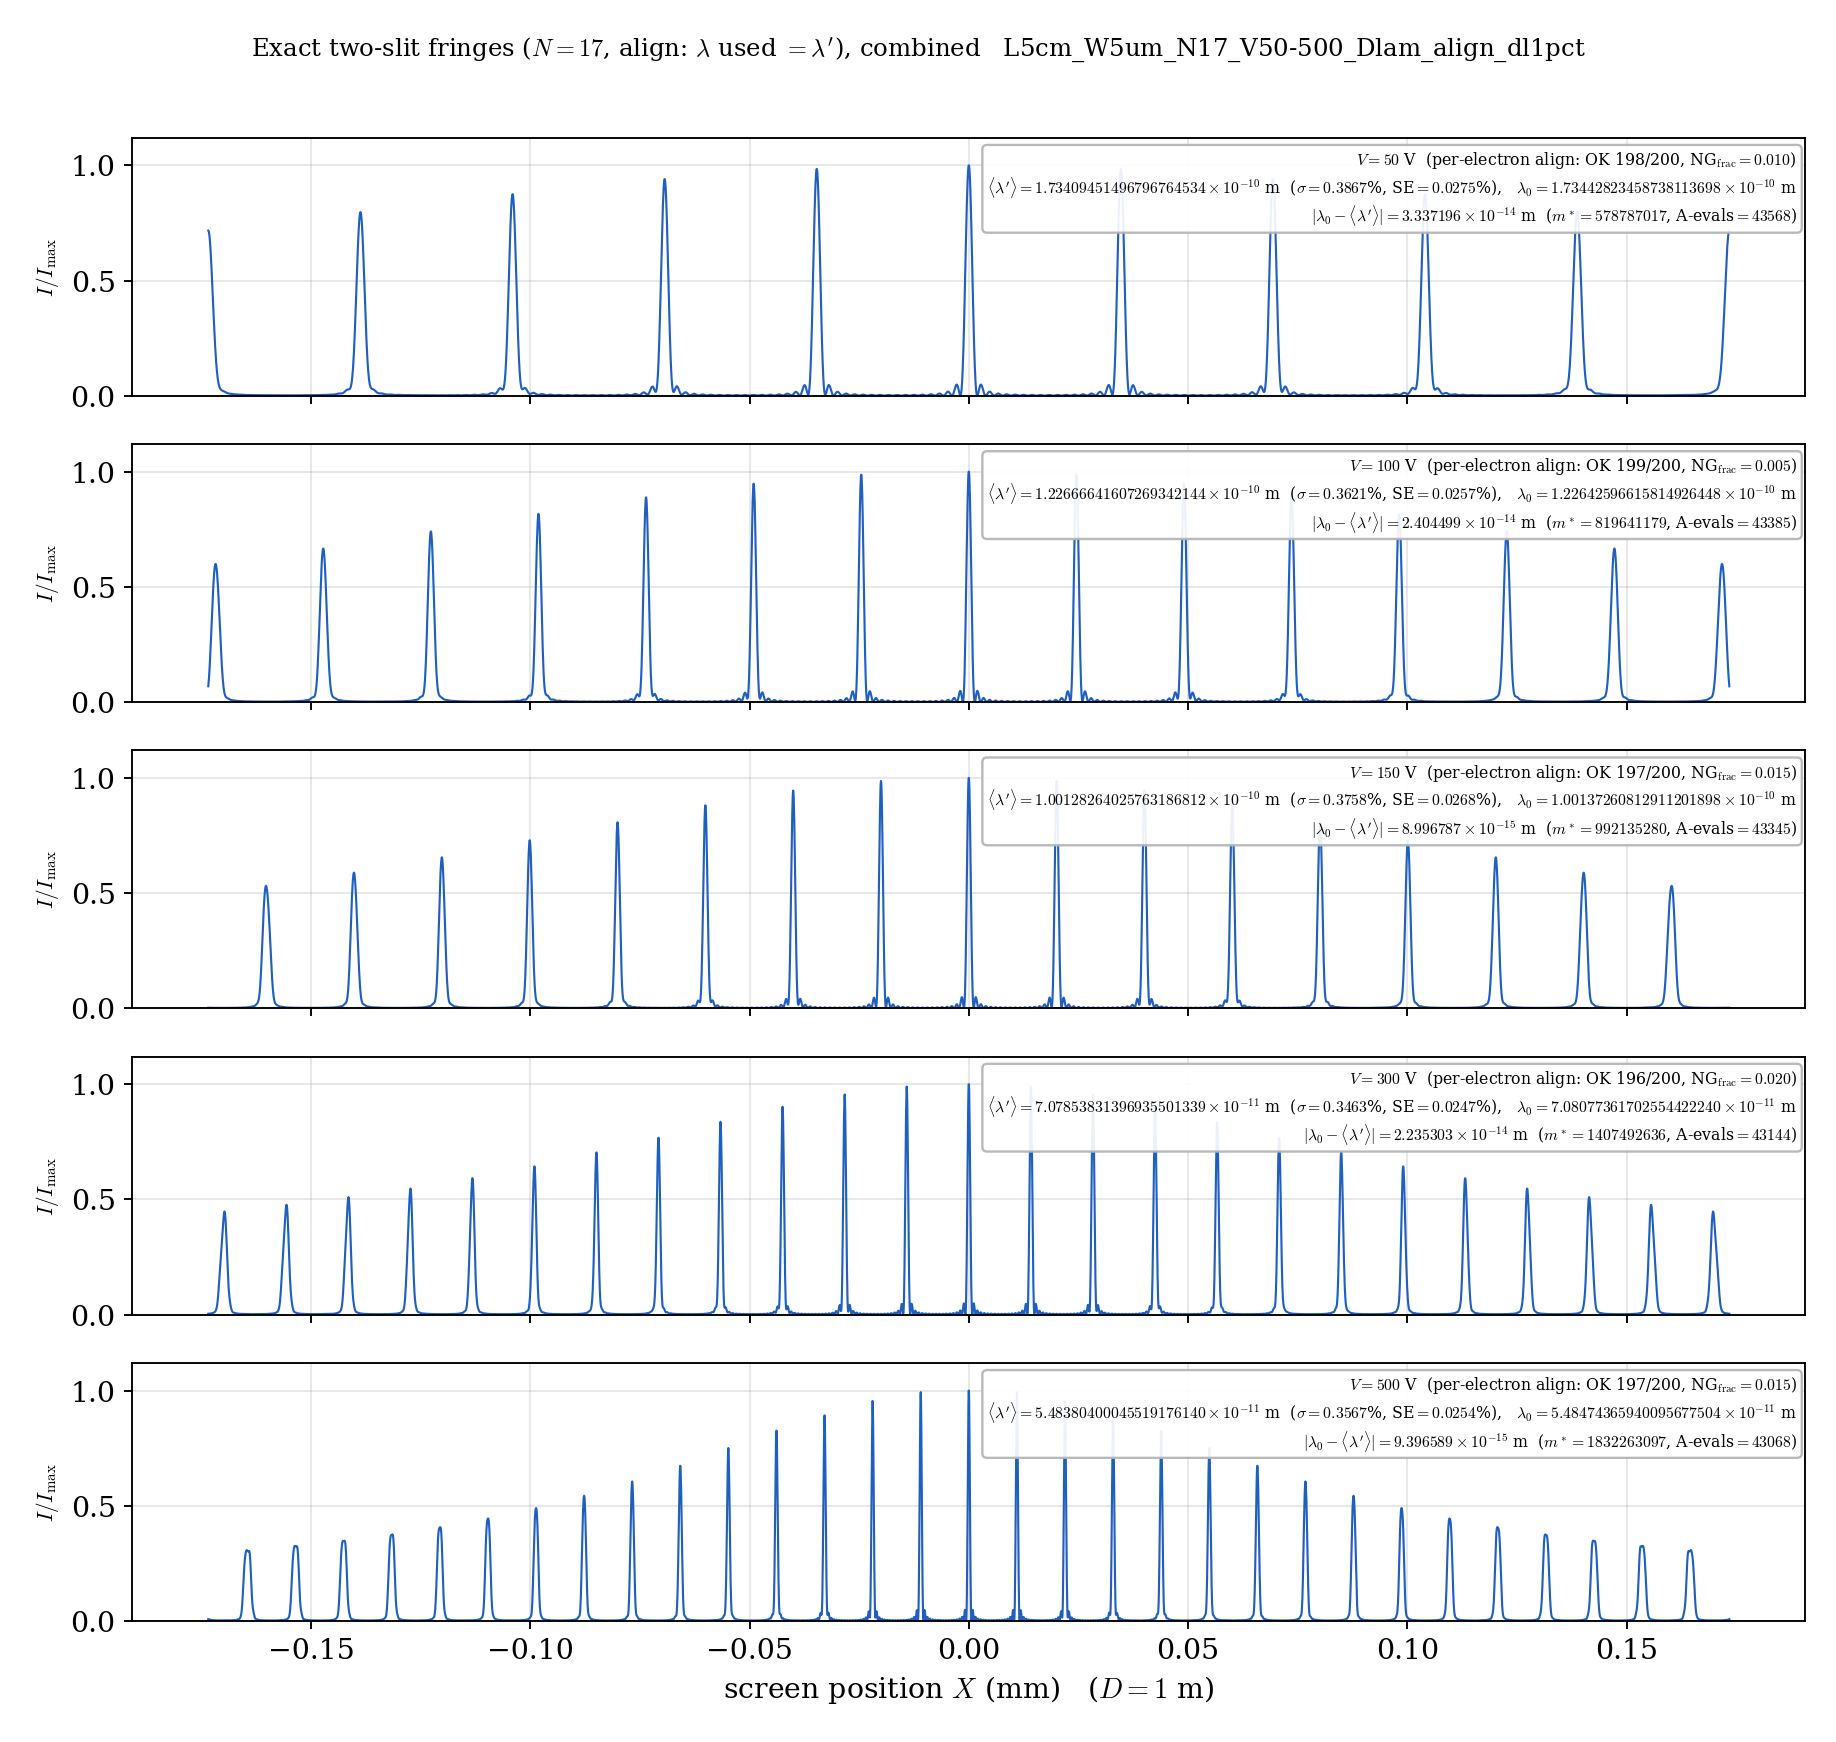
\includegraphics[keepaspectratio,alt={図5}]{debroglie_fringes_combined_L5cm_W5um_N17_V50-500_Dlam_align_dl1pct.png}}
\textbf{図5}:
\(N=17\)・整列。倍音9本でさらに鋭い局在。\textbf{ピーク位置・間隔は
\(N\) によらず不変}で、\(N\) は分解能（鋭さ
\(\sim1/(N{+}1)\)）のみを制御する。

{\def\LTcaptype{none} % do not increment counter
\begin{longtable}[]{@{}
  >{\raggedleft\arraybackslash}p{(\linewidth - 8\tabcolsep) * \real{0.2000}}
  >{\raggedleft\arraybackslash}p{(\linewidth - 8\tabcolsep) * \real{0.2000}}
  >{\raggedleft\arraybackslash}p{(\linewidth - 8\tabcolsep) * \real{0.2000}}
  >{\raggedleft\arraybackslash}p{(\linewidth - 8\tabcolsep) * \real{0.2000}}
  >{\raggedleft\arraybackslash}p{(\linewidth - 8\tabcolsep) * \real{0.2000}}@{}}
\toprule\noalign{}
\begin{minipage}[b]{\linewidth}\raggedleft
\(N\)
\end{minipage} & \begin{minipage}[b]{\linewidth}\raggedleft
倍音数 \(K\)
\end{minipage} & \begin{minipage}[b]{\linewidth}\raggedleft
raw \(\mathrm{slope}/h\)（診断量）
\end{minipage} & \begin{minipage}[b]{\linewidth}\raggedleft
align \(\mathrm{slope}/h\)
\end{minipage} & \begin{minipage}[b]{\linewidth}\raggedleft
局在幅 \(\sim1/(N{+}1)\)
\end{minipage} \\
\midrule\noalign{}
\endhead
\bottomrule\noalign{}
\endlastfoot
1 & 1 & \(0.99977\) & \(0.99977\) & 正弦波（局在なし） \\
9 & 5 & \(0.139\)（崩壊・無効） & \(0.99973\) & \(\sim1/10\) \\
17 & 9 & \(0.081\)（崩壊・無効） & \(0.99972\) & \(\sim1/18\) \\
\end{longtable}
}

\textbf{表1}: 傾き\(/h\) の \(N\) 依存（\(\pm1\%\)
波長揺らぎ・200電子平均）。\textbf{raw
の値は崩壊パターンへの形式的読み取りで、波長測定値ではない}。整列すれば
\(N\) によらず \(\mathrm{slope}/h\approx1\)。

整列後、スクリーン方向の主ピーク位置は \(Ws/\lambda'\in\mathbb{Z}\)
で与えられ、近軸座標 \(X\simeq Ds\) での主ピーク間隔は
\(\Delta X=\lambda' D/W\) となる。奇数倍音数 \(N\)
はピークの鋭さ・サイドローブ構造を変えるが、この\textbf{主ピーク間隔は基本波長
\(\lambda'\) のみで決まり \(N\) に依存しない}。

\textbf{本節の中心的結果（\(\lambda_0\)
の由来によらない構造的結果）}：\(N\) を上げても、align
後の鋭い局在ピーク列の\textbf{間隔（＝中央縞間隔
\(\Delta X=\lambda_0 D/W\)）は基本波長 \(\lambda_0\) で決まり、倍音数
\(N\) によらない}。すなわち、\(\lambda_0\)
より細かい内部構造（倍音）を詰めても、二スリット幾何で観測される波長スケールは基本波長として\textbf{不変}に保たれ、\(N\)
が変えるのは局在の鋭さ（分解能）のみである。\textbf{高
\(N\)＝高分解能かつ高脆弱（許容帯 \(\sim1/(2N)\)）}
のトレードオフは、原子時計や電子干渉計の分解能--安定性トレードオフの古典的アナロジーとして今後比較しうる（本稿では詳細比較はしない）{[}1{]}。

\begin{center}\rule{0.5\linewidth}{0.5pt}\end{center}

\section{\texorpdfstring{5. \(p\) vs \(1/\lambda\) と \(p\lambda\)
一定性の模擬観測}{5. p vs 1/\textbackslash lambda と p\textbackslash lambda 一定性の模擬観測}}\label{p-vs-1lambda-ux3068-plambda-ux4e00ux5b9aux6027ux306eux6a21ux64ecux89b3ux6e2c}

\pandocbounded{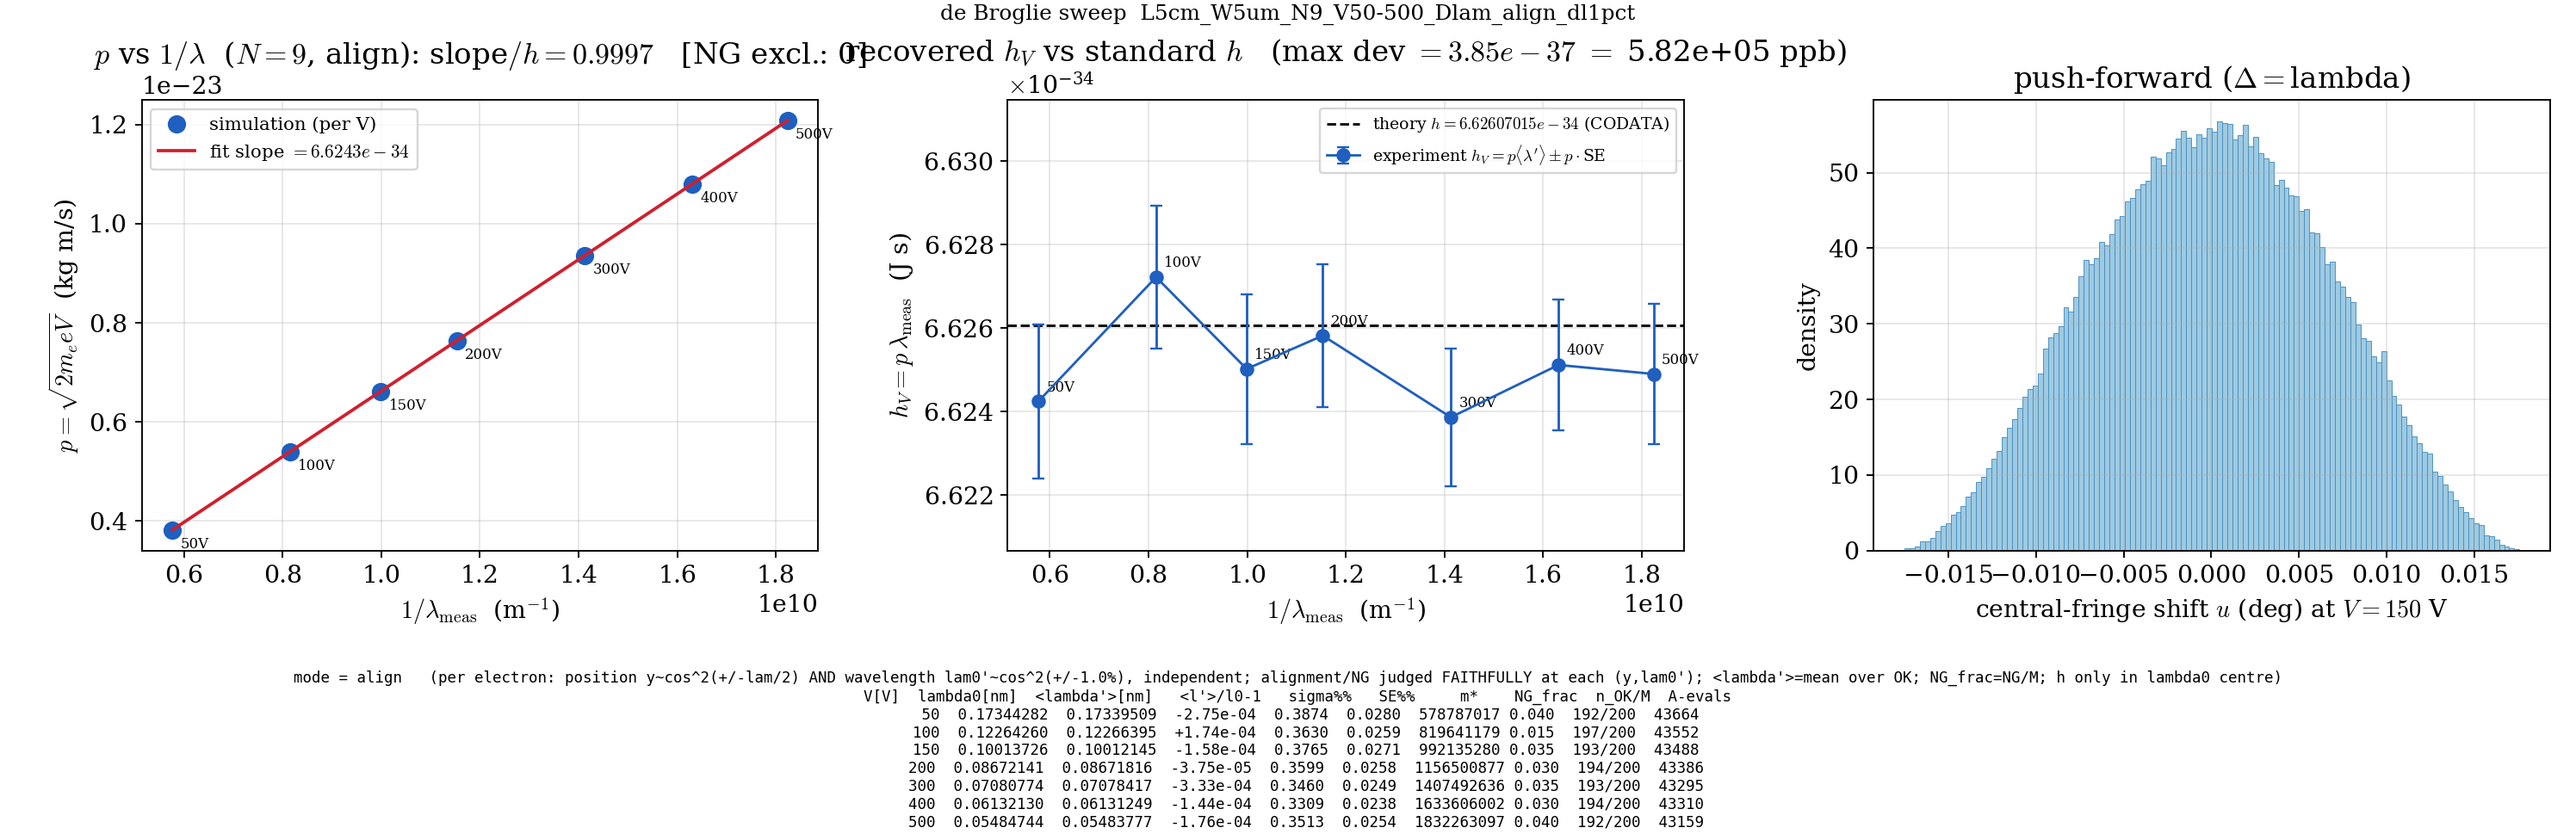
\includegraphics[keepaspectratio,alt={図6}]{debroglie_sweep_L5cm_W5um_N9_V50-500_Dlam_align_dl1pct.png}}
\textbf{図6}: \(N=9\)・整列の総括（\(\pm1\%\) 波長揺らぎ、各電圧 200
電子）。 \textbf{図の読み方（3パネル）}：\textbf{左}＝\(p\) vs
\(1/\langle\lambda'\rangle\)（直線、傾き
\(=h\)）。直線性は関係の可視化であって精度ではない。\textbf{中央}＝各電圧の
\(h_V=p\langle\lambda'\rangle\) を \(\pm p\cdot\)SE
の誤差棒付きで、CODATA
\(h\)（点線・中心）の周りに極端ズームで表示。全点の誤差棒が \(h\)
を含み、\(\langle p\lambda'\rangle\) が \(h\) と統計的に無矛盾（散布
\(\sim0.03\%\)＝\(\pm1\%\)
の200平均）。\textbf{右}＝源位置揺らぎ（\(\cos^2\)）による中央フリンジ位置シフト分布。下部の表に
\(\langle\lambda'\rangle\)、\(\sigma\%\)、SE\(\%\)、除外率、\(n_{\mathrm{OK}}/200\)、\(A\)
評価回数。代表値：\(\sigma\approx0.35\text{–}0.39\%\)（理論 \(0.362\%\)
と一致）、SE \(\approx0.025\text{–}0.028\%\)、除外率
\(1.5\text{–}4.0\%\)、\(n_{\mathrm{OK}}=192\text{–}197/200\)。

\subsection{5.1
自己整合性の明示}\label{ux81eaux5df1ux6574ux5408ux6027ux306eux660eux793a}

各電子の初期波長 \(\lambda_0'\) の\textbf{中心}に \(\lambda_0=h/p\)
を用いている。\(h\)
はこの1箇所で入り、\(\lambda'\approx\lambda_0\)（スナップ
\(\sim10^{-9}\)）を経て \(p\lambda'\approx h\)
として戻る。したがって「\(h\)
を回復する」こと自体は\textbf{自己整合的（自己循環的）}であり、独立な
\(h\) の数値決定ではない。\(\pm1\%\) の波長揺らぎと 200
電子平均は誤読対策の現実性付与であって、多数平均
\(\langle p\lambda'\rangle\to h\) は \(\lambda_0'\) が \(\lambda_0=h/p\)
を中心に対称であることによる相殺の帰結である（干渉が真値 \(h\)
を独立に選別・補正するのではない）。§4
で述べた\textbf{構造の生存と基本波長不変性}は、この自己循環に依存しない別個の結果である。

\subsection{5.2
本稿が導出していないこと（主張の射程）}\label{ux672cux7a3fux304cux5c0eux51faux3057ux3066ux3044ux306aux3044ux3053ux3068ux4e3bux5f35ux306eux5c04ux7a0b}

\textbf{(a) \(p\lambda=h\) の第一原理的導出ではない。}
\(p=\sqrt{2m_eeV}\) は加速電圧から定まる古典運動量（\(h\)
不使用）、\(\lambda\) は波源に与える代表波長 \(\lambda_0=h/p\)
および干渉から抽出される有効波長 \(\lambda'\) である。\(\lambda_0\)
自体が \(h\) を用いて与えられる以上、\(p\lambda'\approx h\)
は自己整合的結果であり、\(p\) と \(\lambda\) の共役性から \(h\)
が現れることを導いたものではない。

\textbf{(b) \(\Delta x\,\Delta p\sim h\) 型不確定性関係の導出ではない。}
本稿の局在奇数倍音波が本質的に持つのは、局在幅 \(\Delta x\) と波数幅
\(\Delta k\) の間の古典波動的（フーリエ的）関係
\(\Delta x\,\Delta k\sim1\) にすぎない。これを運動量幅に接続して
\(\Delta x\,\Delta p\sim\hbar\) を得るには、別途 \(p=\hbar k\)（＝de
Broglie
対応そのもの）を物理的入力として要する。本稿はこれを仮定した前段階であり、不確定性関係を導出しない。

以上より本稿が示すのは、\textbf{de Broglie スケールを代表波長とする波に
\(\lambda_0\)
より細かい局在奇数倍音構造を与えても、二スリット幾何と整列条件のもとで鋭い干渉として安定に生存し、模擬観測される中央縞間隔が基本波長
\(\lambda_0\)
として不変に保たれる}、という古典波動模型としての結果であって、値としての
\(h\) の導出でも、共役性・不確定性の導出でもない。

\subsection{5.3
実実験との対応（限定的アナロジー）}\label{ux5b9fux5b9fux9a13ux3068ux306eux5bfeux5fdcux9650ux5b9aux7684ux30a2ux30caux30edux30b8ux30fc}

Davisson--Germer
等も粗い推定で波長域を追い込んだのち格子干渉で精度を上げるが、実実験では回折角という外部測定データが
\(\lambda\) を独立に与える。本模型は \(\lambda_0=h/p\)
から縞を生成して読み戻すため独立な測定経路を持たず、この点で同型ではない。NG（除外）や
per-electron
整列は、量子測定・波束収縮のモデル化ではなく、古典的な「安定干渉が成立した試行のみを採用する」フィルタリング操作であり、量子古典対応の一具体例として位置づけられる（§2.5,
§7）。

\begin{center}\rule{0.5\linewidth}{0.5pt}\end{center}

\section{6.
計算・模型の限界}\label{ux8a08ux7b97ux6a21ux578bux306eux9650ux754c}

\begin{itemize}
\tightlist
\item
  \textbf{自己参照性}：\(\lambda_0'\) の中心に \(h/p\)
  を用いるため、\(h\) の数値は独立に決まらない。
\item
  \textbf{格子稠密性による自明性}：共鳴格子間隔
  \(\sim10^{-19}\,\mathrm{m}\) が密なため \(\lambda'\approx\lambda_0\)
  は数学的にほぼ必然。本稿の主張は「値の回復」でなく「局在構造の干渉生存と基本波長不変性」に置く（§4,
  §7）。\(L\)
  を大幅に小さくする、または光学波長スケールで類似計算を行えば
  \(\lambda'\) と \(\lambda_0\)
  の乖離が可視化され、機構の非自明性が際立つはずである（今後の課題）。
\item
  \textbf{数値精度}：\(r_{\mathrm{avg}}/\lambda\sim10^9\) ゆえ整列位相は
  float64 の限界にあり、\(A(\lambda)=I(0)/4K^2\)（絶対整列）で計算し
  \(\lambda'=2r_{\mathrm{avg}}/M\) を直接構成して桁落ちを回避している。
\item
  \textbf{次数 \(M\) の非可算性}：\(M\sim10^9\) は Bragg
  回折の小さな次数 \(n=1,2,3\) と異なり縞計数で同定できず、結晶 Bragg
  回折と完全には同型でない。
\item
  \textbf{押し出し効果の微小性}：源位置揺らぎ
  \(\pm\lambda_0/2\)（本稿の基本仮定）に対するフリンジシフトは近軸ゆえ
  \(\sim0.02^\circ\)
  と微小で、中央波長スケールへの寄与は小さい（仮定の下での正しい帰結）。
\item
  \textbf{代表値}：\(L,W,V,\Delta,\delta\)
  は代表値であり、定量精度は限定的である。
\end{itemize}

\begin{center}\rule{0.5\linewidth}{0.5pt}\end{center}

\section{7. 結論と展望}\label{ux7d50ux8ad6ux3068ux5c55ux671b}

単一源ダブルスリットの古典波動模型において、de Broglie
スケールの代表波長 \(\lambda_0=h/p\)
を持つ局在奇数倍音波（\(N>1\)）に、各電子ごと位置（\(\pm\lambda_0/2\)）と波長（\(\pm1\%\)）を独立に揺らがせて厳密に干渉・整列・除外判定を行った。\(N=1\)
は手続きの検算にあたる。\textbf{本稿の中心的結果は \(h\)
の値ではなく、(i) \(\lambda_0\)
より細かい局在構造を持つ古典波が二スリット幾何で鋭い単一ピーク干渉として安定に生存できること、(ii)
生存した縞の中央間隔が基本波長 \(\lambda_0\) のまま倍音数 \(N\)
によらず不変に保たれること（\(N\) は分解能 \(\sim1/(N{+}1)\)
のみ制御）}である。中心波長を \(\lambda_0=h/p\) とする対称揺らぎのもとで
\(\langle p\lambda'\rangle\) は標準誤差の範囲で \(h\)
と一致するが、これは格子稠密性による自己整合であって独立導出ではない。

\textbf{本稿の結果は \(p\lambda=h\)
の第一原理的導出でも、\(\Delta x\,\Delta p\sim h\)
型不確定性の導出でもない。} 本稿の価値は「\(h\)
を導出した」ことではなく、\textbf{de Broglie
波長より小さい局在構造を持たせても、観測される干渉波長が de Broglie
スケールとして残る（基本波長不変性）ことを、明示的な古典波動模型で検証した}ことにある。

展望：(a) 粗格子 regime（小 \(L\) ／光学波長）で
\(\lambda'\ne\lambda_0\) を可視化し機構の非自明性を示す、(b) 除外率の
\(N\)・揺らぎ幅 \(\delta\) 依存の定量化、(c)
整列鋭敏性（高分解能かつ高脆弱）の原子時計・電子干渉計との普遍構造としての位置づけ、(d)
英語版の公開。

\begin{center}\rule{0.5\linewidth}{0.5pt}\end{center}

\section{参考文献}\label{ux53c2ux8003ux6587ux732e}

{[}1{]} N. Kihara,
\emph{単一源ダブルスリット模型における局在奇数倍音波と整列条件（Localized
odd-harmonic wave and the alignment condition in a single-source
double-slit model）}, Zenodo (2026). DOI:
\href{https://doi.org/10.5281/zenodo.21035831}{10.5281/zenodo.21035831}.（※正確な題名・DOI・公開状態は当該
deposit で確定すること）

{[}2{]} C. Davisson and L. H. Germer, ``Diffraction of Electrons by a
Crystal of Nickel,'' \emph{Physical Review} \textbf{30}, 705--740
(1927). DOI: 10.1103/PhysRev.30.705.

{[}3{]} L. de Broglie, ``Recherches sur la théorie des quanta,''
\emph{Annales de Physique} \textbf{10}(3), 22--128 (1925). DOI:
10.1051/anphys/192510030022.（正式誌面情報・DOI を最終確認すること）

{[}4{]} M. Born, ``Zur Quantenmechanik der Stoßvorgänge,''
\emph{Zeitschrift für Physik} \textbf{37}, 863--867 (1926). DOI:
10.1007/BF01397477. --- 本稿では源位置分布に用いた \(\cos^2\)
型確率密度を \textbf{Born 型（\(|\psi|^2\)
型）確率分布の仮定}として参照する（§2.4）。Born
則そのものを導出・適用するものではない。

\begin{center}\rule{0.5\linewidth}{0.5pt}\end{center}

\emph{付記：数値・図は、パラメータ化した
\texttt{debroglie\_plambda\_sweep.py}（厳密二スリット強度＋位置・波長の独立
\(\cos^2\) 揺らぎ＋per-electron 積算）と、絶対整列 \(A\) 探索ソルバ
\texttt{debroglie\_align\_lambda.py}
により生成した。図の生成条件はファイル名に符号化されている（例：\texttt{...\_N9\_V50-500\_Dlam\_align\_dl1pct}＝\(N{=}9\)・整列・波長揺らぎ
\(\pm1\%\)）。}
\end{document}
